\begin{wrapfigure}{r}{0.5\linewidth}
  \begin{center}
    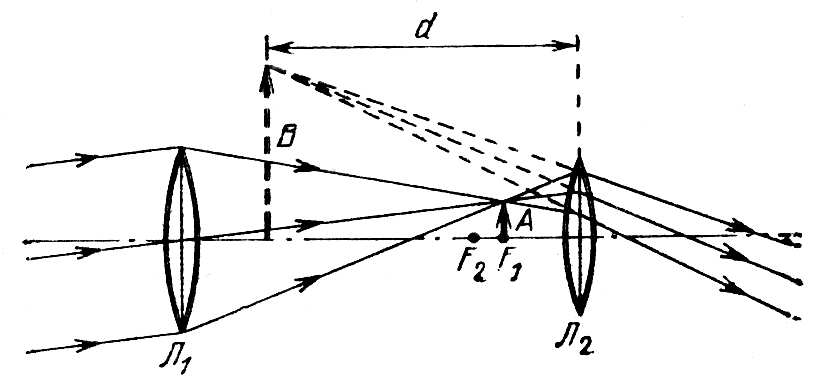
\includegraphics[width=0.8\linewidth]{1.png}
  \end{center}
  \caption{Ход лучей в трубе Кеплера}
  \label{img::1}
  \begin{center}
    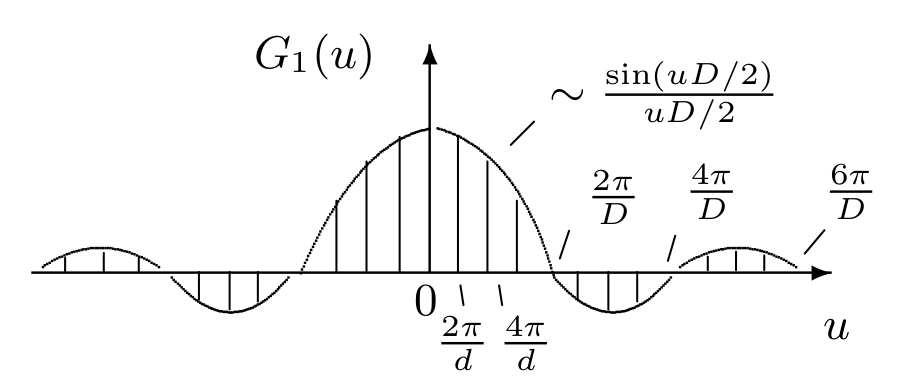
\includegraphics[width=0.8\linewidth]{2.png}
  \end{center}
  \caption{Ход лучей в трубе Галилея}
  \label{img::2}
  \begin{center}
    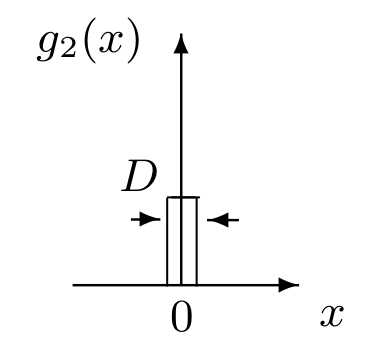
\includegraphics[width=0.8\linewidth]{3.png}
  \end{center}
  \caption{Ход лучей в микроскопе}
  \label{img::3}
\end{wrapfigure}

В настоящей работе изучаются модели зрительных труб (астрономической и земной) и микроскопа. 
Каждый из этих оптических приборов состоит из двух основных частей: объектива -- линзы, 
обращённой к объекту, и окуляра -- линзы, обращённой к наблюдателю. Объектив, в качестве 
которого используется положительная линза, создаёт действительное изображение предмета. 
Это изображение рассматривается глазом через окуляр. Ход лучей в астрономической
и земной зрительных трубах и в микроскопе представлен на рис. \ref{img::1}, \ref{img::2}, \ref{img::3}.

Поскольку зрительные трубы используются для наблюдения удалённых предметов, находящихся
от объектива на расстояниях, значительно превышающих его фокусное расстояние, изображение
$A$ предмета, даваемое объективом, находится практически в его фокальной плоскости. В 
случае микроскопа промежуточное изображение $A$ находится далеко за фокальной плоскостью
объектива, так как предмет располагается вблизи переднего фокуса.

Мнимое изображение $B$, даваемое окуляром, располагается на некотором расстоянии $d$ от 
окуляра. Наводя оптический инструмент на резкость, наблюдатель автоматически устанавливает
такое расстояние $d$, которое удобно для аккомодации глаза. Поскольку глаз обладает 
значительной областью аккомодации 1, расстояние $d$ даже для одного и того же наблюдателя
может существенно изменяться от опыта к опыту. При изменении аккомодации оптический прибор, 
вооружающий глаз, должен быть несколько перефокусирован. В зрительных трубах этого достигают 
перемещением окуляра, а в микроскопе -- перемещением всей оптической системы относительно 
предмета. Для того чтобы исключить в теории произвол, связанный с неопределённостью 
расстояния $d$, полагают обычно, что глаз наблюдателя аккомодирован на бесконечность.
При этом мнимое изображение $B$ должно располагаться в бесконечности, и, следовательно,
промежуточное изображение $A$ должно совпадать с фокальной плоскостью окуляра.

При наблюдении предметов с помощью зрительной трубы или микроскопа угловой размер 
изображения, рассматриваемого глазом, оказывается существенно больше, чем угловой размер 
объекта при наблюдении невооружённым глазом. Отношение углового размера изображения 
объекта, рассматриваемого наблюдателем через окуляр прибора, к угловому размеру объекта, 
рассматриваемого невооружённым глазом, называется угловым увеличением оптического прибора. 
При этом в случае микроскопа полагают, что при непосредственном наблюдении расстояние 
между объектом и глазом равно расстоянию наилучшего зрения глаза, т.е. 25 см. В случае 
зрительной трубы всегда предполагается, что расстояние между объектом и наблюдателем 
значительно превышает фокусное расстояние объектива.